
\section{Ejercicio 1 Opcional}
\begin{tcolorbox}[colback=yellow!5!white,colframe=yellow!75!black]
    \textit{Cuando se hace referencia a la imagen X, se refiere a la imagen 2.X(hasta el punto de Firewall)}
  
\end{tcolorbox}

El alumno/a debe ser capaz de presentar un MV con la configuración descrita en este apartado. La configuración debe ser permanente, es decir, en todo caso, tras reiniciar el equipo, la configuración será la esperada.
Para validar la configuración de red, el alumno/a debe ser capaz de:
\begin{itemize}
    \item Hacer ping desde el equipo anfitrión a la MV y viceversa.
    \item Hacer ping desde la MV a cualquier equipo accesible públicamente en Internet por FQHN o IP.
    \item Conectar por ssh desde el equipo anfitrión a la MV .
\end{itemize}

\subsection{Solución}
Una vez que hayamos instalado el SO que se nos pide correctamente. Debemos de realizar una serie de ajustes previos:
\begin{itemize}
    \item Añadir nuestro usuario, para ello debemos de ejecutar lo siguientes comandos (iniciando como usuario root):
    \begin{itemize}
        \item \texttt{sudo useradd nombre\_de\_usuario}        
        \item \texttt{sudo passwd nombre\_de\_usuario}
        \item \texttt{sudo usermod -aG wheel nombre\_de\_usuario} para que pueda usar el comando sudo.
    \end{itemize}
\end{itemize}

\begin{itemize}
    \item Configurar la red NAT y una de tipo Host-Only, para ello en Herramientas en la VM debemos seleccionar la opción de Red y añadir una nueva interfaz de red de tipo Host-Only, y paso seguido configurar la red NAT (ver Figura 1 y 2 )
    \item Comprobar que el servicio SSH está instalado, por defecto se suele instalar, para asegurarnos debemos de ejecutar el comando \texttt{sudo systemctl status ssh}. En el caso de que no venga instalado debemos de ejecutar el comando \texttt{sudo dnf install -y openssh-server openssh-clients}\footnote{Incluimos clients para añadir el servicio de cliente.} (Ver Figura 5).
    \item Cambiar la variable PS1 como se nos pedía, para ello debemos de editar el fichero de bashrc y exportar la variable PS1 con el valor que se nos pedía:
    \begin{itemize}
        \item \texttt{PS1='\textbackslash u@\textbackslash h:\textbackslash t:\textbackslash w\textbackslash\$ '} (Ver Figura 5), donde:
        \begin{itemize}
            \item \texttt{\textbackslash u}: Nombre del usuario actual.
            \item \texttt{\textbackslash h}: Nombre del hostname (nombre del sistema).
            \item \texttt{\textbackslash t}: Hora actual en formato de 24 horas (HH:MM:SS).
            \item \texttt{\textbackslash w}: Directorio de trabajo actual.
            \item \texttt{\$}: Símbolo del prompt, que será \$ para un usuario normal y \# para root.
        \end{itemize}
    \end{itemize}
\end{itemize}

\begin{figure}[htbp]
    \centering
    \begin{minipage}[b]{0.45\textwidth}
        \centering
        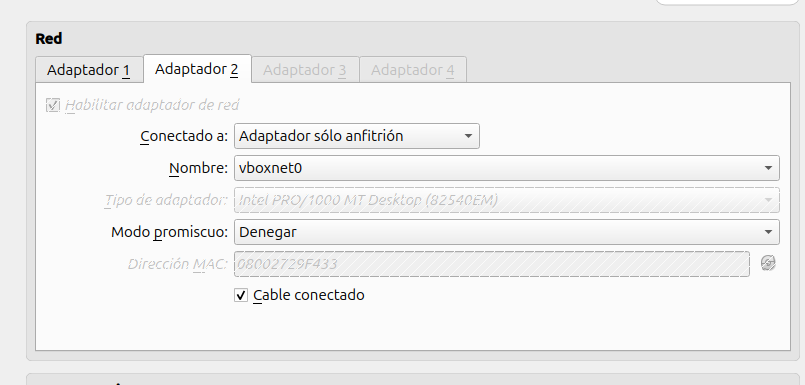
\includegraphics[width=\textwidth]{images/Bloque1/adaptador2.png}
        \caption{Configuración de la red NAT y Host-Only}
    \end{minipage}
    \hfill
    \begin{minipage}[b]{0.45\textwidth}
        \centering
        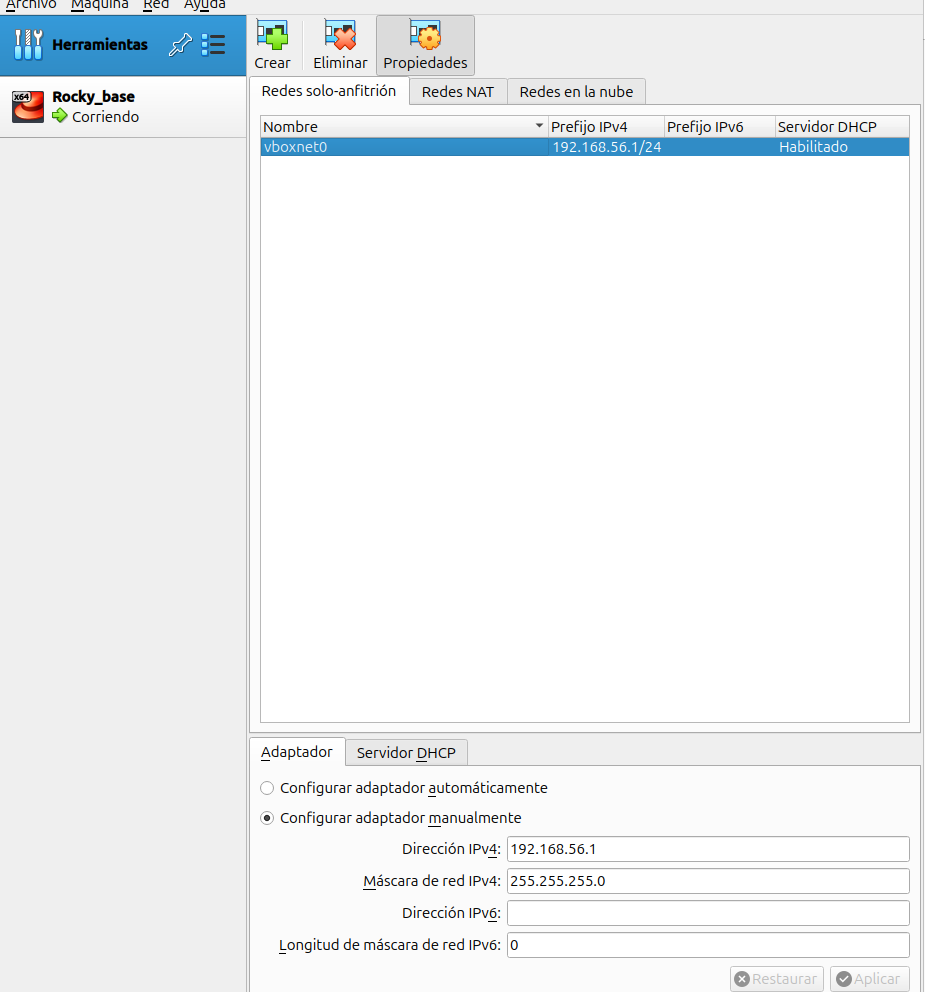
\includegraphics[width=\textwidth]{images/Bloque1/vbox.png}
        \caption{Configuración de VirtualBox para la red de Host-Only}
    \end{minipage}
\end{figure}

Además se nos pide que la Ip de Host Only sea estática, para ello vamos a asegurarnos usando la herramienta \textit{nmtui}, en la que vamos a ver si es estática o no la ip. Como podemos ver en la siguiente imagen esta configurada como ip automática, que viene siendo lo mismo que dinámica por lo que debemos de cambiarlo a manual para poder configurar la ip estática. (Ver Figura 3 y 4). Para ver que efectivamente la ip cambió, podemos verlo en la Figura 5.
\begin{figure}[htbp]
    \centering
    \begin{minipage}[b]{0.45\textwidth}
        \centering
        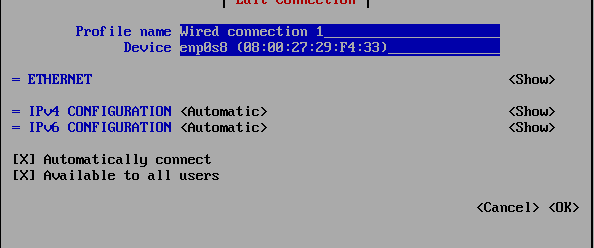
\includegraphics[width=\textwidth]{images/Bloque1/nmtui1.png}
        \caption{Con nmtui vemos que es dinámica}
    \end{minipage}
    \hfill
    \begin{minipage}[b]{0.45\textwidth}
        \centering
        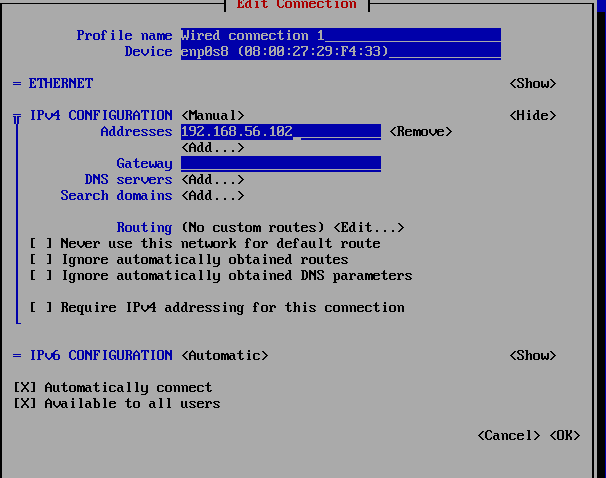
\includegraphics[width=\textwidth]{images/Bloque1/nmtui_2.png}
        \caption{Cambiamos a manual y asignamos una ip estática válida}
    \end{minipage}
\end{figure}



\begin{figure}
    \centering
    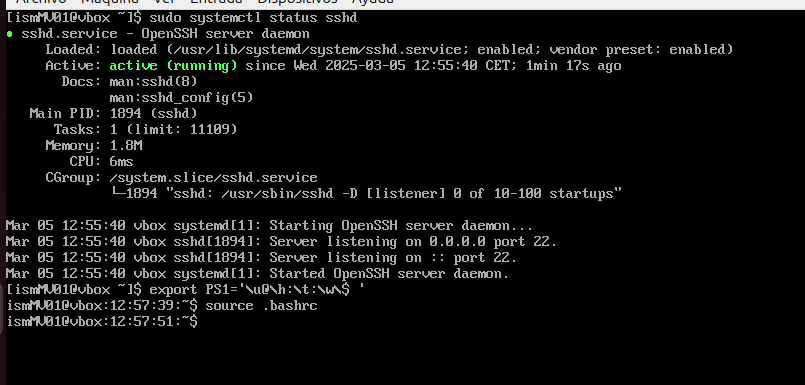
\includegraphics[width=0.8\textwidth]{images/Bloque1/sshd_PS1.png}
    \caption{Sshd y variable PS1}
\end{figure}

\begin{figure}
    \centering
    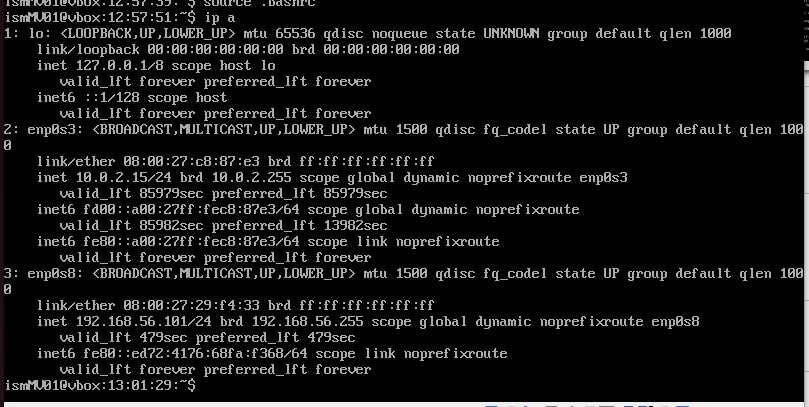
\includegraphics[width=0.8\textwidth]{images/Bloque1/resultado_ipa.png}
    \caption{Resultado de ip a}
\end{figure}

Una vez hayamos cambiado la ip estática, debemos de verificar que efectivamente se ha cambiado y para ello usamos el comando \texttt{ip a} y vemos que efectivamente se ha cambiado la ip a la que hemos asignado. (Ver Figura 7).

\begin{figure}
    \centering
    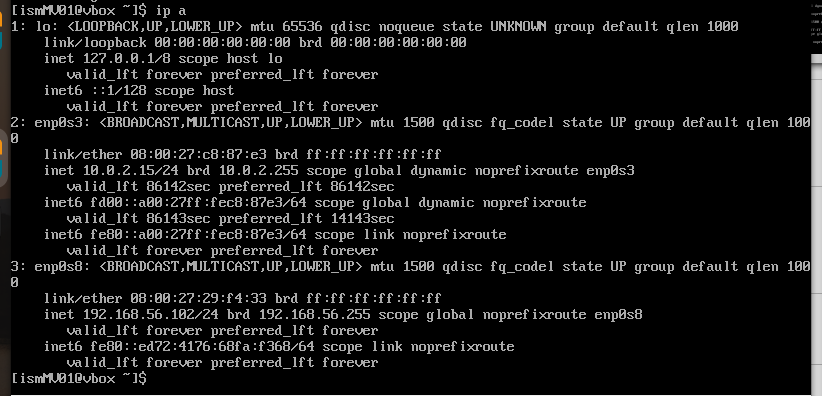
\includegraphics[width=0.8\textwidth]{images/Bloque1/ping2.png}
    \caption{Resultado de ip a para verificar el cambio de ip}
\end{figure}

Llegado a este punto vamos a realizar un ping a la máquina anfitriona y viceversa, para ello usamos el comando \texttt{ping -c <número de pings> ip\_de\_la\_maquina} y vemos que efectivamente hay conexión entre ambas máquinas. (Ver Figura 8, 9 y 10). Además, vemos que gracias al \textit{NAT} podemos hacer ping a cualquier máquina accesible en internet\footnote{Cabe destacar que durante el desarrollo de la actividad, surgían algunas problemas con NetworkManager, polkiy y DBus, pero se solucionaban al reiniciarlos o bien reinstalarlos}. (Ver Figura 11).

\begin{figure}[htbp]
    \centering
    \begin{minipage}[b]{0.45\textwidth}
        \centering
        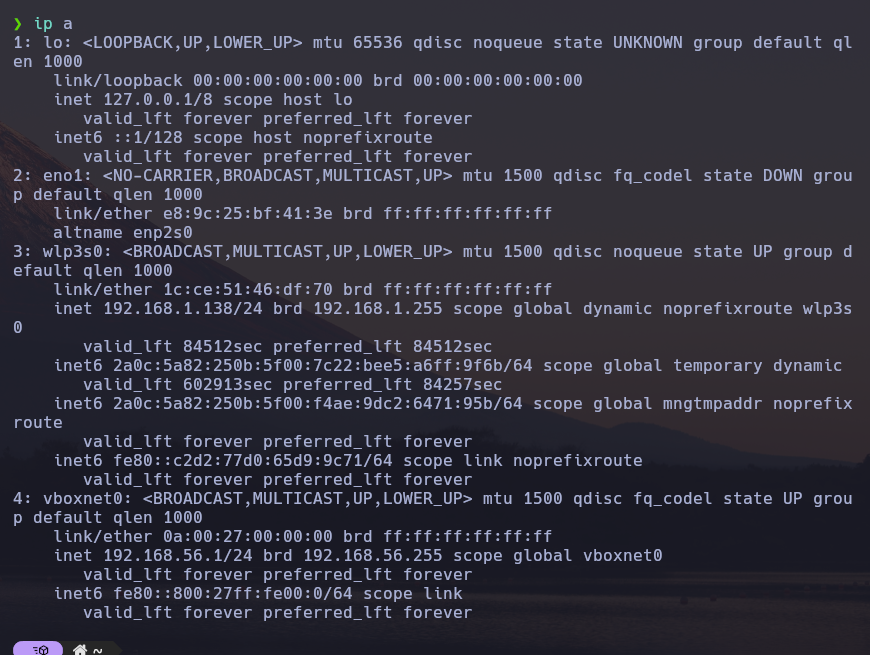
\includegraphics[width=\textwidth]{images/Bloque1/ip_a_host.png}
        \caption{Resultado del comando de \textit{ip a } en la máquina anfitriona para ver la ip}
    \end{minipage}
    \hfill
    \begin{minipage}[b]{0.45\textwidth}
        \centering
        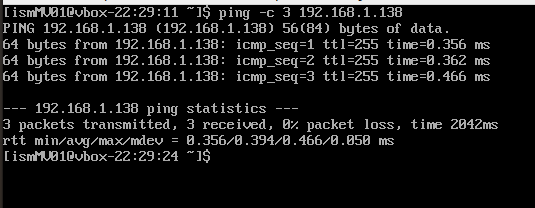
\includegraphics[width=\textwidth]{images/Bloque1/ping_a_anfitriona.png}
        \caption{Ping a la máquina anfitriona}
    \end{minipage}
\end{figure}


\begin{figure}[htbp]
    \centering
    \begin{minipage}[b]{0.45\textwidth}
        \centering
        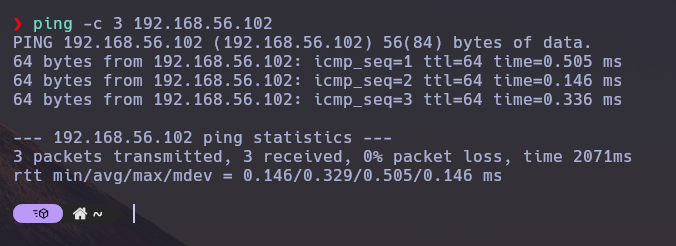
\includegraphics[width=\textwidth]{images/Bloque1/ping_anf_a_mv.png}
        \caption{Ping de la máquina anfitriona a la máquina virtual}
    \end{minipage}
    \hfill
    \begin{minipage}[b]{0.45\textwidth}
        \centering
        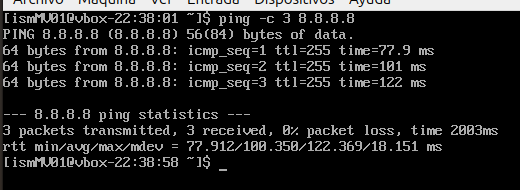
\includegraphics[width=\textwidth]{images/Bloque1/ping_fuera.png}
        \caption{Ping a un servidor público (Google)}
    \end{minipage}
\end{figure}


En cuanto al servicio ssh, debemos de ver el estado del servicio sshd con el comando \texttt{sudo systemctl status sshd} y vemos que esta corriendo. En este punto desde el anfitrión podemos introducirt la línea de comando \texttt{ssh ismMV01@192.168.56.102} y vemos que efectivamente todo funciona correctamente. (Ver Figura 12 y 13).






\begin{figure}[htbp]
    \centering
    \begin{minipage}[b]{0.45\textwidth}
        \centering
        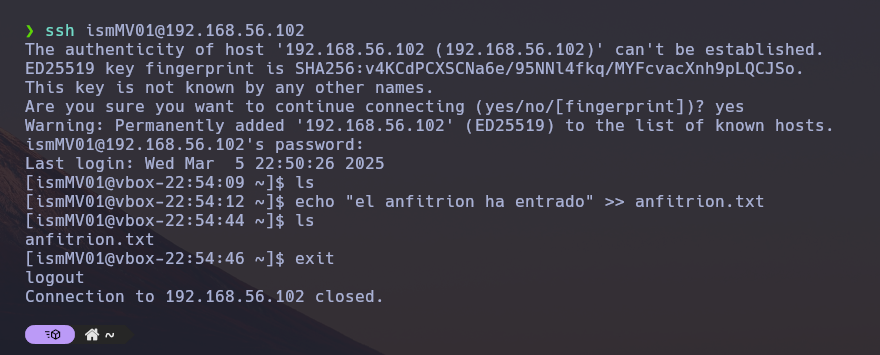
\includegraphics[width=\textwidth]{images/Bloque1/ssh1.png}
        \caption{Ssh en la máquina anfitriona y creación de un archivo en la MV}
    \end{minipage}
    \hfill
    \begin{minipage}[b]{0.45\textwidth}
        \centering
        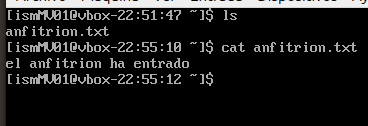
\includegraphics[width=\textwidth]{images/Bloque1/ssh2.png}
        \caption{Ver el contenido del archivo creado en la MV desde el anfitrión}
    \end{minipage}
\end{figure}
\newpage
\section{Servidor con LVM + RAID}

\subsection{Aspectos clave de LVM}

Para gestionar eficazmente el \textit{Logical Volume Manager} (LVM), es fundamental comprender los siguientes componentes y conceptos:

\subsubsection{Componentes de la arquitectura de almacenamiento}

\begin{itemize}
  \item \textbf{Physical Volume (PV)}: Representa los dispositivos de almacenamiento físico, como discos duros o particiones, que se incorporan al sistema LVM.
  \item \textbf{Volume Group (VG)}: Es una agrupación de uno o más PVs que forman un pool de almacenamiento, del cual se pueden asignar espacios para crear volúmenes lógicos.
  \item \textbf{Logical Volume (LV)}: Son volúmenes virtuales creados dentro de un VG. Los LVs se utilizan como si fueran particiones de disco tradicionales, permitiendo la creación de sistemas de archivos o la asignación directa a aplicaciones.
\end{itemize}

\subsubsection{Gestión de almacenamiento con diferentes características físicas}

LVM ofrece flexibilidad para manejar dispositivos de almacenamiento con diversas características físicas:

\begin{itemize}
  \item \textbf{HDD y SSD}: Se pueden combinar en un mismo VG, permitiendo equilibrar rendimiento y capacidad según las necesidades.
  \item \textbf{RAID}: LVM puede trabajar sobre dispositivos RAID, proporcionando una capa adicional de gestión y flexibilidad sobre la configuración RAID existente.
\end{itemize}

\subsubsection{Etiquetado y correspondencia con los archivos de dispositivo}

Cada componente en LVM tiene una nomenclatura específica y se asocia a archivos de dispositivo en el sistema:

\begin{itemize}
  \item \textbf{Physical Volumes}: Corresponden a dispositivos físicos, como \texttt{/dev/sda1}, \texttt{/dev/sdb1}, etc.
  \item \textbf{Volume Groups}: Se nombran según la convención establecida por el administrador, por ejemplo, \texttt{vg\_datos}.
  \item \textbf{Logical Volumes}: Se nombran dentro de su VG correspondiente, como \textit{/dev/vg\_datos/lv\_backup}, donde \textit{lv\_backup} es el nombre del LV.
\end{itemize}

\subsubsection{Comandos de LVM para la gestión de componentes}

LVM proporciona una serie de comandos para administrar sus componentes:

\begin{itemize}
  \item \texttt{pvcreate}: Inicializa un dispositivo físico como PV.
  \item \texttt{vgcreate}: Crea un VG a partir de uno o más PVs.
  \item \texttt{lvcreate}: Crea un LV dentro de un VG.
  \item \texttt{pvs}, \texttt{vgs}, \texttt{lvs}: Muestran información sobre PVs, VGs y LVs respectivamente.
  \item \texttt{pvremove}, \texttt{vgremove}, \texttt{lvremove}: Eliminan PVs, VGs y LVs respectivamente.
\end{itemize}

Estos comandos permiten una gestión eficiente y flexible del almacenamiento en sistemas que utilizan LVM.

\subsection{Niveles de RAID: 0, 1 y 5}

Redundant Array of Independent Disks (RAID) es una tecnología que permite combinar múltiples dispositivos de almacenamiento en una unidad lógica para mejorar el rendimiento, la redundancia o ambos. A continuación, se detallan los niveles de RAID 0, 1 y 5, sus ventajas, desventajas y su administración en sistemas Linux utilizando la herramienta de línea de comandos \texttt{mdadm}.

\subsubsection{RAID 0}

RAID 0, conocido como \textit{striping}, distribuye los datos de manera equitativa entre dos o más discos sin información de paridad ni redundancia.

\begin{itemize}
  \item \textbf{Ventajas}:
    \begin{itemize}
      \item Mayor rendimiento en lectura y escritura debido a la distribución de datos entre los discos.
      \item Uso completo de la capacidad de almacenamiento total, ya que no se reserva espacio para paridad o duplicación.
    \end{itemize}
  \item \textbf{Desventajas}:
    \begin{itemize}
      \item Ausencia de redundancia; la falla de un solo disco resulta en la pérdida total de los datos.
    \end{itemize}
\end{itemize}

\subsubsection{RAID 1}

RAID 1, o \textit{mirroring}, duplica los datos en dos o más discos, creando copias idénticas en cada uno.

\begin{itemize}
  \item \textbf{Ventajas}:
    \begin{itemize}
      \item Alta redundancia; los datos permanecen intactos incluso si uno de los discos falla.
      \item Mejora en la velocidad de lectura, ya que los datos pueden leerse desde cualquiera de los discos.
    \end{itemize}
  \item \textbf{Desventajas}:
    \begin{itemize}
      \item Capacidad de almacenamiento efectiva reducida al 50\% del total, ya que los datos se duplican.
    \end{itemize}
\end{itemize}

\subsubsection{RAID 5}

RAID 5 combina rendimiento y redundancia distribuyendo los datos y la paridad entre tres o más discos.

\begin{itemize}
  \item \textbf{Ventajas}:
    \begin{itemize}
      \item Proporciona tolerancia a fallos; si un disco falla, los datos pueden recuperarse con la información de paridad.
      \item Mejor aprovechamiento del almacenamiento comparado con RAID 1, ya que solo se utiliza una fracción del espacio para la paridad.
    \end{itemize}
  \item \textbf{Desventajas}:
    \begin{itemize}
      \item Rendimiento de escritura inferior al de RAID 0 debido al cálculo de la paridad.
      \item En caso de falla de un disco, la reconstrucción puede ser lenta y afectar el rendimiento.
    \end{itemize}
\end{itemize}

\subsubsection{Administración de RAID en Linux con mdadm}

La herramienta \texttt{mdadm} permite gestionar arreglos RAID en Linux. A continuación, se presentan comandos esenciales:

\begin{itemize}
  \item Crear un RAID 0 con dos discos:
    \begin{lstlisting}[style=mystyle][style=mystyle]
    mdadm --create --verbose /dev/md0 --level=0 --raid-devices=2 /dev/sdX /dev/sdY
    \end{lstlisting}
  \item Crear un RAID 1 con dos discos:
    \begin{lstlisting}[style=mystyle][style=mystyle]
    mdadm --create --verbose /dev/md0 --level=1 --raid-devices=2 /dev/sdX /dev/sdY
    \end{lstlisting}
  \item Crear un RAID 5 con tres discos:
    \begin{lstlisting}[style=mystyle][style=mystyle]
    mdadm --create --verbose /dev/md0 --level=5 --raid-devices=3 /dev/sdX /dev/sdY /dev/sdZ
    \end{lstlisting}
  \item Verificar el estado del RAID:
    \begin{lstlisting}[style=mystyle][style=mystyle]
    cat /proc/mdstat
    \end{lstlisting}
  \item Detener un RAID:
    \begin{lstlisting}[style=mystyle][style=mystyle]
    mdadm --stop /dev/md0
    \end{lstlisting}
\end{itemize}

\subsection{Aspectos clave para la administración de servidores Linux}

Para implementar eficazmente soluciones en servidores Linux, es esencial comprender y manejar los siguientes aspectos:

\subsubsection{Modos de ejecución y modo de mantenimiento en un servidor Linux}

Los sistemas Linux operan en diferentes niveles de ejecución o \textit{runlevels}, que determinan los servicios y procesos que se ejecutan. Con la adopción de \textit{systemd}, estos niveles se denominan \textit{targets}. El modo de mantenimiento, conocido como \textit{rescue.target} o \textit{emergency.target}, es crucial para tareas de recuperación y administración del sistema. Para cambiar al modo de mantenimiento, se puede utilizar el siguiente comando:

\begin{lstlisting}[style=mystyle][style=mystyle]
sudo systemctl isolate rescue.target
\end{lstlisting}

Para volver al modo multiusuario estándar:

\begin{lstlisting}[style=mystyle][style=mystyle]
sudo systemctl isolate multi-user.target
\end{lstlisting}

\subsubsection{Estructura estándar del sistema de archivos en Linux}

La estructura de directorios en Linux sigue el estándar de jerarquía de sistemas de archivos (\textit{Filesystem Hierarchy Standard - FHS}). Algunos directorios principales incluyen:

\begin{itemize}
  \item \textbf{/}: Directorio raíz que contiene todos los demás directorios.
  \item \textbf{/bin}: Ejecutables esenciales para todos los usuarios.
  \item \textbf{/etc}: Archivos de configuración del sistema.
  \item \textbf{/home}: Directorios personales de los usuarios.
  \item \textbf{/var}: Datos variables como registros y colas de impresión.
\end{itemize}

\subsubsection{Sistemas de archivos comunes en Linux}

Linux soporta diversos sistemas de archivos. Algunos de los más comunes son:

\begin{itemize}
  \item \textbf{ext4}: Sistema de archivos por defecto en muchas distribuciones, conocido por su estabilidad y rendimiento.
  \item \textbf{XFS}: Adecuado para manejar grandes volúmenes de datos y archivos de gran tamaño.
  \item \textbf{Btrfs}: Ofrece características avanzadas como instantáneas (\textit{snapshots}) y compresión.
\end{itemize}

\subsubsection{Montaje y desmontaje de volúmenes}

El montaje de sistemas de archivos permite acceder a dispositivos de almacenamiento. Para montar un dispositivo:

\begin{lstlisting}[style=mystyle][style=mystyle]
sudo mount /dev/sdX1 /mnt/punto_de_montaje
\end{lstlisting}

Para desmontarlo:

\begin{lstlisting}[style=mystyle][style=mystyle]
sudo umount /mnt/punto_de_montaje
\end{lstlisting}

Las configuraciones de montaje persistentes se definen en el archivo \texttt{/etc/fstab}.

\subsubsection{Comandos básicos para la gestión de archivos}

La administración de archivos en Linux se realiza mediante comandos de línea. 


% Algunos comandos fundamentales incluyen:

% \begin{itemize}
%   \item \texttt{cp}: Copiar archivos o directorios.
%     \begin{lstlisting}[style=mystyle][style=mystyle]
%     cp origen destino
%     \end{lstlisting}
%   \item \texttt{mv}: Mover o renombrar archivos o directorios.
%     \begin{lstlisting}[style=mystyle][style=mystyle]
%     mv origen destino
%     \end{lstlisting}
%   \item \texttt{rm}: Eliminar archivos.
%     \begin{lstlisting}[style=mystyle][style=mystyle]
%     rm archivo
%     \end{lstlisting}
%   \item \texttt{mkdir}: Crear un nuevo directorio.
%     \begin{lstlisting}[style=mystyle][style=mystyle]
%     mkdir nombre_del_directorio
%     \end{lstlisting}
%   \item \texttt{ls}: Listar el contenido de un directorio.
%     \begin{lstlisting}[style=mystyle][style=mystyle]
%     ls ruta_del_directorio
%     \end{lstlisting}
%   \item \texttt{cat}: Mostrar el contenido de un archivo.
%     \begin{lstlisting}[style=mystyle][style=mystyle]
%     cat archivo
%     \end{lstlisting}
%   \item \texttt{nano} o \texttt{vim}: Editores de texto para modificar archivos desde la terminal.
%     \begin{lstlisting}[style=mystyle][style=mystyle]
%     nano archivo
%     \end{lstlisting}
% \end{itemize}

% Estos comandos son esenciales para la gestión diaria de archivos y directorios en un entorno Linux.
Estos se deben de haber estudiado en asignaturas anteriores como Sistemas Operativos.

\subsection{Ejercicio Opcional}

Partiendo de un servidor básico configurado de acuerdo al apartado 2, el alumno/a deberá
afrontar el caso práctico descrito a continuación:

Se desea instalar un servicio de gestión documental en el servidor. Se espera que este servicio
precise de una cantidad espacio de almacenamiento creciente con el tiempo, pudiendo llegar a
ser considerable.

Por otro lado, el contenido será crítico, por lo que se desea proporcionar
algún mecanismo de respaldo ante fallos en el dispositivo de almacenamiento.

El alumno/a debe diseñar los cambios en el sistema de almacenamiento e implementarlo
empleando prácticas adecuadas de administración que garanticen la conservación de la
información en el sistema y procuren la máxima disponibilidad del servicio.

\subsubsection{Solución}

Para la resolución de este ejercicio vamos a seguir lo realizado en clase. (Ver apuntes de clase correspondientes a la sección de LVM+RAID).

En primer lugar creamos los discos, para ello entramos en la configuración de la máquina virtual y añadimos dos discos duros de 1GB cada uno. Una vez añadidos los discos duros, iniciamos la máquina virtual y ejecutamos el comando \texttt{lsblk} para ver los discos duros que tenemos disponibles. (Ver Figura 14).

\begin{figure}[htbp]
  \centering
  \begin{minipage}[b]{0.45\textwidth}
      \centering
      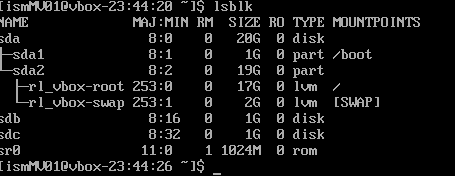
\includegraphics[width=\textwidth]{images/Bloque1/lsblk.png}
      \caption{Resultado del comando lsblk}
  \end{minipage}
  \hfill
  \begin{minipage}[b]{0.45\textwidth}
      \centering
      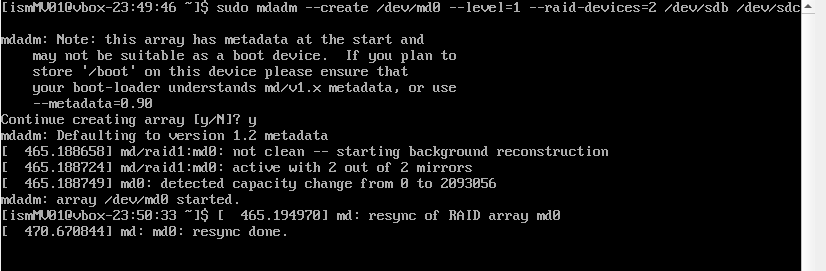
\includegraphics[width=\textwidth]{images/Bloque1/mdadm.png}
      \caption{Comando mdadm}
  \end{minipage}
\end{figure}

A continuación, instalamos \textit{mdadm} con el comando \texttt{sudo dnf install -y mdadm} y creamos un RAID 1 con los dos discos duros que hemos añadido. Para ello ejecutamos el comando \texttt{sudo mdadm --create --verbose /dev/md0 --level=1 --raid-devices=2 /dev/sdb /dev/sdc} y vemos que se ha creado correctamente. (Ver Figura 15).

Acto seguido debemos de crear un PV, VG y LV. Para ello ejecutamos los siguientes comandos (Ver Figura 16):
\begin{itemize}
  \item \texttt{sudo pvcreate /dev/md0}
  \item \texttt{sudo vgcreate vg\_datos /dev/md0}
  \item \texttt{sudo lvcreate -L 900M -n lv\_datos vg\_datos}
\end{itemize}

\begin{figure}[htbp]
  \centering
  \begin{minipage}[b]{0.45\textwidth}
      \centering
      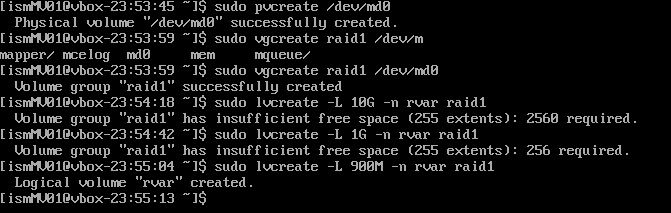
\includegraphics[width=\textwidth]{images/Bloque1/create.png}
      \caption{Resultado de crear los volúmenes}
  \end{minipage}
  \hfill
  \begin{minipage}[b]{0.45\textwidth}
      \centering
      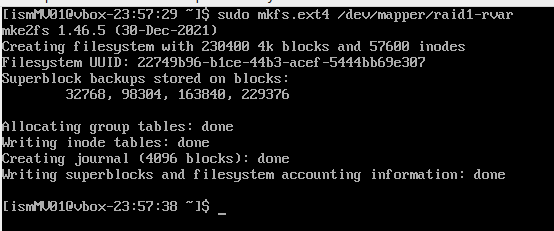
\includegraphics[width=\textwidth]{images/Bloque1/mkfs.png}
      \caption{Comando mkfs}
  \end{minipage}
\end{figure}

Ahora debemos de formatear el volumen lógico en formato ext4. (Ver Figura 17).

A continuación, montamos (Ver Figura 18) y trasladamos la carpeta \textit{var} al nuevo volumen lógico. Para ello ejecutamos los comando que figuran en los apuntes de clase.

\begin{figure}[htbp]
  \centering
  \begin{minipage}[b]{0.45\textwidth}
      \centering
      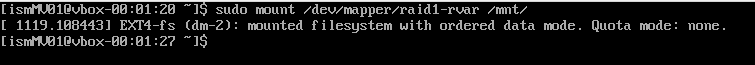
\includegraphics[width=\textwidth]{images/Bloque1/mount.png}
      \caption{Resultado del comando mount}
  \end{minipage}
  \hfill
  \begin{minipage}[b]{0.45\textwidth}
      \centering
      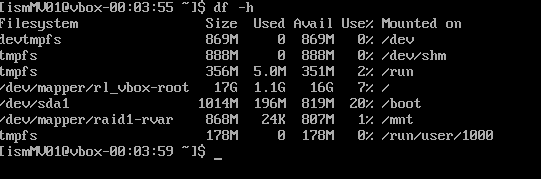
\includegraphics[width=\textwidth]{images/Bloque1/df.png}
      \caption{Comando df -h}
  \end{minipage}
\end{figure}

  Ejecutamos el comando \texttt{df -h} para ver que efectivamente se ha montado correctamente el volumen lógico. (Ver Figura 19).

  Ejecutamos el isolate del systemctl para entrar en modo de mantenimiento y poder trasladar la carpeta \textit{var} al nuevo volumen lógico. (Ver Figura 20).

  \begin{figure}[htbp]
    \centering
    \begin{minipage}[b]{0.45\textwidth}
        \centering
        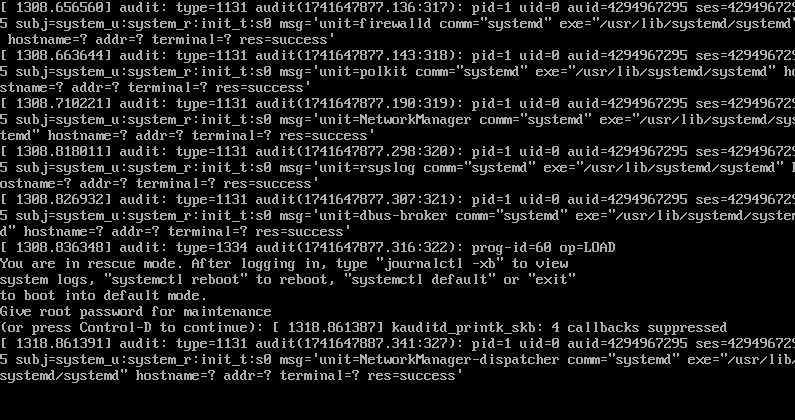
\includegraphics[width=\textwidth]{images/Bloque1/isolate.png}
        \caption{Resultado del comando systemctl isolate}
    \end{minipage}
    \hfill
    \begin{minipage}[b]{0.45\textwidth}
        \centering
        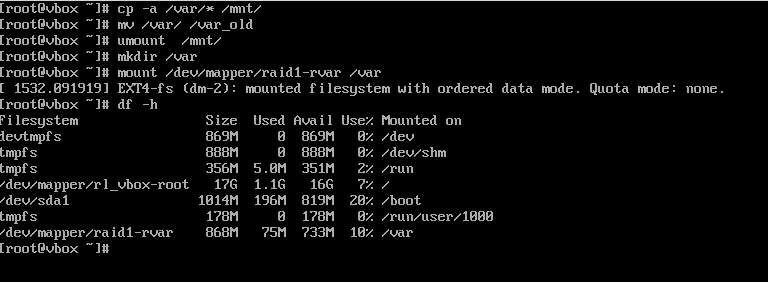
\includegraphics[width=\textwidth]{images/Bloque1/var.png}
        \caption{Serie de operaciones para trasladar la carpeta var}
    \end{minipage}
  \end{figure}

Ahora debemos de trabajar con la serie de comandos que se especifican para poder mover la carpeta y que se haga de forma correcta. (Ver Figura 21).

Una vez trasladad la carpeta, debemos de hacer permanentes los cambios, para ello debemos de editar el fichero \texttt{/etc/fstab} y añadir la siguiente línea (Ver Figura 22):

\begin{lstlisting}[style=mystyle][style=mystyle]
  /dev/mapper/raid1-rvar /var ext4 defaults 0 0
\end{lstlisting}

Recargamos la configuraciones con el deamon de systemd y vemos que aparece la parte que estabamos montando (Ver Figura 23).

\begin{figure}[htbp]
  \centering
  \begin{minipage}[b]{0.45\textwidth}
      \centering
      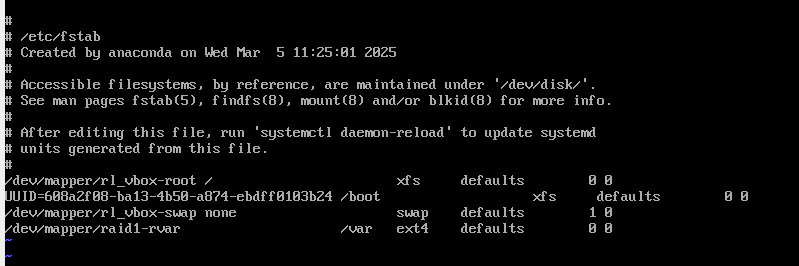
\includegraphics[width=\textwidth]{images/Bloque1/fstab.png}
      \caption{Resultado de editar /etc/fstab como se indica}
  \end{minipage}
  \hfill
  \begin{minipage}[b]{0.45\textwidth}
      \centering
      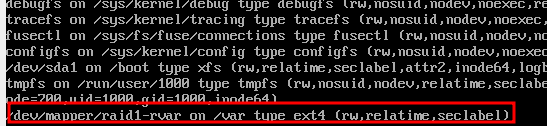
\includegraphics[width=\textwidth]{images/Bloque1/daemon.png}
      \caption{Resultado del comando systemctl daemon-reload y mount}
  \end{minipage}
\end{figure}

Y como podemos comprobar en la Figura 24, hemos conseguido trasladar la carpeta \textit{var} al nuevo volumen lógico y todo funciona correctamente.

\begin{figure}[H]
  \centering
  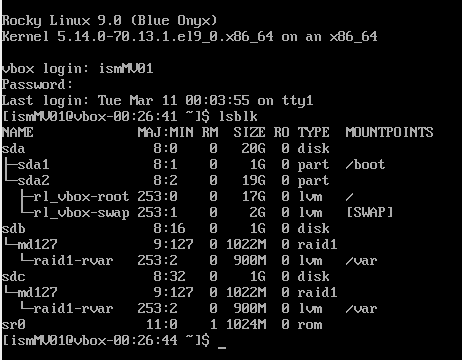
\includegraphics[width=0.6\textwidth]{images/Bloque1/resultadofinal_raid.png}
  \caption{Resultado final}
\end{figure}

\newpage
\section{Acceso seguro al servidor: Firewall + SSHD}

\subsection{Iptables}

\texttt{iptables} es una herramienta de línea de comandos utilizada para configurar el cortafuegos en el núcleo de Linux, implementado dentro del proyecto Netfilter. Aunque \texttt{iptables} es un marco heredado, \texttt{nftables} se presenta como su reemplazo moderno, ofreciendo una capa de compatibilidad. 

\subsubsection{Instalación}

El núcleo estándar de Arch Linux viene compilado con soporte para \texttt{iptables}. Para instalar las utilidades de usuario, se debe instalar el paquete \texttt{iptables}, que es una dependencia indirecta del metapaquete \texttt{base}, por lo que debería estar instalado por defecto en el sistema. 

\subsubsection{Conceptos Básicos}

\begin{itemize}
    \item \textbf{Tablas}: Colecciones de reglas con propósitos específicos.
    \item \textbf{Cadenas}: Listas de reglas dentro de una tabla que se recorren en orden.
    \item \textbf{Reglas}: Definiciones que consisten en un criterio de coincidencia y una acción a ejecutar si se cumple dicho criterio.
\end{itemize}

\subsubsection{Configuración y Uso}

\texttt{iptables} se puede configurar directamente desde la línea de comandos o mediante diversas interfaces frontales, tanto de consola como gráficas. Para mostrar las reglas actuales, se utiliza:

\begin{verbatim}
iptables -L
\end{verbatim}

Para restablecer las reglas:

\begin{verbatim}
iptables -F
\end{verbatim}

\subsubsection{Registro de Actividad}

\texttt{iptables} permite registrar paquetes para monitorear actividad o depurar reglas. Es posible limitar la tasa de registro para evitar la saturación de los registros del sistema. 
\subsubsection{Alternativas y Herramientas Relacionadas}

\begin{itemize}
    \item \textbf{\texttt{nftables}}: Proyecto que busca reemplazar a \texttt{iptables}, proporcionando un nuevo marco de filtrado de paquetes y una utilidad de espacio de usuario llamada \texttt{nft}. 
    \item \textbf{\texttt{ipset}}: Aplicación complementaria que permite crear conjuntos de direcciones IP para ser utilizados en reglas de \texttt{iptables}, facilitando el bloqueo o la aceptación de múltiples direcciones de manera eficiente. 
    \item \textbf{\texttt{ufw} (Uncomplicated Firewall)}: Programa para gestionar el cortafuegos de manera sencilla, proporcionando una interfaz de línea de comandos fácil de usar. 
\end{itemize}

\subsubsection{Recursos Adicionales}

Para configuraciones más avanzadas, como la creación de un cortafuegos con estado o compartir la conexión a Internet, se pueden consultar las siguientes guías:

\begin{itemize}
    \item \textbf{Cortafuegos con Estado Sencillo}: Explica cómo configurar un cortafuegos con estado utilizando \texttt{iptables}, detallando las reglas necesarias y su propósito. 
    \item \textbf{Compartir Conexión a Internet}: Describe cómo compartir la conexión a Internet desde una máquina a otras, incluyendo los requisitos y pasos necesarios.
\end{itemize}


\subsection{firewalld y firewall-cmd en Rocky Linux}

\texttt{firewalld} es un servicio de cortafuegos dinámico que permite gestionar reglas de firewall sin necesidad de reiniciar el servicio. Su herramienta de línea de comandos, \texttt{firewall-cmd}, proporciona una interfaz para la administración del firewall en sistemas como Rocky Linux.

\subsubsection{Gestión del Firewall con firewall-cmd}

\texttt{firewall-cmd} permite configurar reglas de firewall de manera flexible y en tiempo real. Algunas de las operaciones más comunes incluyen:

\begin{itemize}
    \item \textbf{Verificar el estado del firewall}:
    \begin{verbatim}
    firewall-cmd --state
    \end{verbatim}

    \item \textbf{Listar las reglas activas}:
    \begin{verbatim}
    firewall-cmd --list-all
    \end{verbatim}

    \item \textbf{Abrir un puerto específico} (ejemplo: puerto 80 TCP):
    \begin{verbatim}
    firewall-cmd --add-port=80/tcp --permanent
    \end{verbatim}
    
    \item \textbf{Cerrar un puerto específico}:
    \begin{verbatim}
    firewall-cmd --remove-port=80/tcp --permanent
    \end{verbatim}

    \item \textbf{Recargar la configuración del firewall} para aplicar cambios:
    \begin{verbatim}
    firewall-cmd --reload
    \end{verbatim}
\end{itemize}

\subsubsection{Administración del Servicio firewalld con systemctl}

\texttt{systemctl} es una herramienta utilizada para gestionar servicios en sistemas basados en \texttt{systemd}, como Rocky Linux. Se puede utilizar para controlar el servicio \texttt{firewalld} de la siguiente manera:

\begin{itemize}
    \item \textbf{Verificar si el servicio está activo}:
    \begin{verbatim}
    systemctl status firewalld
    \end{verbatim}

    \item \textbf{Iniciar el servicio} si está detenido:
    \begin{verbatim}
    systemctl start firewalld
    \end{verbatim}

    \item \textbf{Detener el servicio} si se necesita desactivarlo temporalmente:
    \begin{verbatim}
    systemctl stop firewalld
    \end{verbatim}

    \item \textbf{Habilitar el servicio para que se inicie automáticamente} al arrancar el sistema:
    \begin{verbatim}
    systemctl enable firewalld
    \end{verbatim}

    \item \textbf{Deshabilitar el servicio para evitar su inicio automático}:
    \begin{verbatim}
    systemctl disable firewalld
    \end{verbatim}
\end{itemize}

\subsubsection{Verificación de Configuración con nmap}

\texttt{nmap} es una herramienta de escaneo de redes que permite verificar los puertos abiertos y configuraciones de firewall. Se puede usar para comprobar la efectividad de las reglas de firewall aplicadas. Algunos ejemplos de uso incluyen:

\begin{itemize}
    \item \textbf{Escanear los puertos abiertos de una dirección IP específica}:
    \begin{verbatim}
    nmap <direccion_ip>
    \end{verbatim}

    \item \textbf{Escanear puertos específicos} (ejemplo: puertos 22 y 80):
    \begin{verbatim}
    nmap -p 22,80 <direccion_ip>
    \end{verbatim}

    \item \textbf{Detectar el sistema operativo del host analizado}:
    \begin{verbatim}
    nmap -O <direccion_ip>
    \end{verbatim}
\end{itemize}

Estas herramientas permiten una administración avanzada del firewall en Rocky Linux, garantizando la seguridad de la red y el control del tráfico de red en el sistema.

\subsection{Ejercicio Opcional}

Como caso práctico, partiendo de una MV con la configuración base descrita en el apartado 2, el
alumno/a deberá ser capaz de instalar un servidor de HTTP, Apache o Nginx,
y habilitar/deshabilitar su acceso por Firewall.

Para ello, instalará el servidor web de su elección y modificará la home page para mostrar un
mensaje:'Bienvenidos a la web de <Nombre y Apellidos del alumno/a> en Prácticas ISE'.

El servicio web debe estar accesible en la servidor (MV) en el puerto por defecto (80) usando un
navegador web convencional corriendo en el anfitrión (Host).

Un escaneo de puertos sobre el servidor solo debe mostrar como accesibles los puerto web y ssh.

\subsection*{Solución}

Para la resolución de este ejercicio vamos a seguir los siguientes pasos:

\begin{enumerate}
  \item Instalamos el servidor web Apache con el comando \micode{sudo dnf install -y httpd}. También tenemos la opción de instalar Nginx con el comando \micode{sudo dnf install nginx- y}. \textit{Tenemos libre elección de servidor web, en mi caso será Apache}.
  \item Debemos de activar este servicio con el comando:
  \begin{itemize}
    \item Apache: \micode{sudo systemctl enable httpd --now}
    \item Nginx: \micode{sudo systemctl enable nginx --now}
  \end{itemize}
  \item Debemos de verificar que el servicio esta activo con los comandos:
  \begin{itemize}
    \item \micode{sudo systemctl status httpd # Para Apache}
    \item \micode{sudo systemctl status nginx # Para Nginx}
  \end{itemize}
  \item Modificación de la página principal.\\
  Debemos de personalizar la página de inicio de nuestra web para que muestre el mensaje que se nos pide en el enunciado.
  \begin{itemize}
    \item Apache: \micode{echo "Bienvenidos a la web de <Nombre y Apellidos> en Prácticas ISE" | sudo tee /var/www/html/index.html}
    \item Nginx: \micode{echo "Bienvenidos a la web de <Nombre y Apellidos> en Prácticas ISE" | sudo tee /usr/share/nginx/html/index.html}
  \end{itemize}
  \item Configuración del Firewall.\\
  Para permitir el acceso a la web, es necesario abrir el puerto 80 en el firewall. Para ello, ejecutamos los siguientes comandos:
  \begin{itemize}
    \item \micode{sudo firewall-cmd --add-service=http --permanent}
    \item \micode{sudo firewall-cmd --reload}
    \item Para verificar que el puerto esta abierto: \micode{sudo firewall-cmd --list-all}
  \end{itemize}
  \item Acceder desde el Navegador.\\
  Si todo está configurado correctamente, se visualizará el mensaje personalizado\footnote{Para saber a que ip acceder, podemos usar el comando \textit{ip a} y coger la correspondiente a \textit{enp0s8.}}(Ver Figura \ref{web}).
  \begin{figure}[H]
    \centering
      
\includegraphics[width=0.7\textwidth]{images/Bloque1/web.png}
      \caption{Acceso a la web desde el navegador}
      \label{web}
  \end{figure}
  \item Restricción de puertos con Firewall.\\
  Para asegurar que solo los puertos web (80) y SSH (22) estén accesibles, se deben eliminar
otras reglas de firewall:
\begin{itemize}
  \item \micode{sudo firewall-cmd --list-services --permanent}\footnote{Con este comando podemos ver los servicios que están activos en el firewall, desactivamos todos, a excepción de http y ssh.}
  \item \micode{sudo firewall-cmd --remove-service=<nombre> --permanent}
  \item \micode{sudo firewall-cmd --reload}
  \item Extra.\\
  Como extra podemos ver los puertos que están abiertos con el comando \micode{sudo firewall-cmd --list-ports --permanent
  } y cerramos el puerto con \micode{sudo firewall-cmd --remove-port=xxxx/tcp --permanent
  }, donde xxxx es el puerto que queremos cerrar. Otra forma de solo tener dos puertos abiertos es con los comandos:
  \begin{itemize}
    \item \micode{sudo firewall-cmd --add-service=http --permanent}
    \item \micode{sudosudo firewall-cmd --add-service=ssh --permanent}
    \item Y de nuevo recargamos y listamos todos los puertos.
  \end{itemize}
\end{itemize}
\end{enumerate}

\newpage
\section{SSH}

\subsection{Administración remota con SSH y criptografía asimétrica}

La administración remota es una tarea fundamental en la gestión de servidores. Una de las herramientas más utilizadas para este propósito es \texttt{SSH} (Secure Shell), que permite acceder y administrar un sistema de manera segura a través de una red. Es importante destacar que \texttt{SSH} puede referirse tanto a un cliente como a un servicio.

\subsubsection{Instalación y configuración de SSH}
Para instalar y habilitar el servicio SSH en un sistema basado en Rocky Linux, se utilizan los siguientes comandos:

\begin{lstlisting}[style=mystyle]
sudo dnf install -y openssh-server
sudo systemctl enable --now sshd
\end{lstlisting}

El servicio \texttt{sshd} es el demonio que permite las conexiones SSH entrantes. Su configuración se encuentra en el archivo:

\begin{lstlisting}[style=mystyle]
/etc/ssh/sshd_config
\end{lstlisting}

Al editar este archivo, es posible modificar diversas opciones de seguridad, como:

\begin{itemize}
    \item \textbf{Deshabilitar el acceso como root por contraseña:} Para mejorar la seguridad, se recomienda restringir el acceso directo de root:
    \begin{lstlisting}[style=mystyle]
    PermitRootLogin no
    \end{lstlisting}
    
    \item \textbf{Cambio de puerto predeterminado:} SSH por defecto usa el puerto 22, pero puede cambiarse para reducir ataques automatizados:
    \begin{lstlisting}[style=mystyle]
    Port 2222
    \end{lstlisting}
\end{itemize}

Después de modificar la configuración, es necesario reiniciar el servicio:

\begin{lstlisting}[style=mystyle]
sudo systemctl restart sshd
\end{lstlisting}

\subsubsection{Configuración del firewall para SSH}
Si se cambia el puerto de \texttt{SSH}, es necesario actualizar la configuración del firewall:

\begin{lstlisting}[style=mystyle]
sudo firewall-cmd --add-port=2222/tcp --permanent
sudo firewall-cmd --reload
\end{lstlisting}

\subsubsection{Criptografía simétrica y asimétrica en SSH}
\textbf{Criptografía simétrica} es un método en el que la misma clave se usa tanto para cifrar como para descifrar los datos. Es rápida pero menos segura para la comunicación remota, ya que ambas partes deben compartir la clave de forma segura.

\textbf{Criptografía asimétrica}, utilizada en SSH, emplea un par de claves: una clave pública y una clave privada. El cliente genera un par de claves y comparte la clave pública con el servidor, lo que permite autenticarse sin necesidad de enviar una contraseña.

Para generar un par de claves en SSH, se usa:

\begin{lstlisting}[style=mystyle]
ssh-keygen -t rsa -b 4096
\end{lstlisting}

Y para copiar la clave pública al servidor:

\begin{lstlisting}[style=mystyle]
ssh-copy-id usuario@servidor
\end{lstlisting}

Esto permite autenticarse sin necesidad de contraseña, mejorando la seguridad y facilitando la automatización de tareas en servidores remotos.

\subsection{Ejercicio Opcional}

Partiendo de un servidor base configurado siguiendo las indicaciones del apartado 2, el
alumno/a modificará servicio SSHD para que, en lugar del puerto por defecto (22), se ejecute en
un puerto alternativo de un valor mayor a 1024. Se recomienda que consulte la lista de puertos
reconocidos por el sistema en /etc/ports para evitar emplear un puerto que ya tenga una
aplicación predefinida.

Se concederá acceso remoto por llave pública a un usuario de su elección.
El ejercicio se validará ejecutando un comando de forma remota sobre el servidor SSH con la
nueva configuración. El comando presentará el contenido completo (incluido ficheros y
directorios ocultos) con del directorio home del usuario remoto empleado en la conexión. Para
ello, desde el ordenador anfitrión (o una MV distinta a la que se va a acceder) se empleará ssh
sin terminal remoto y sin contraseña, pasando como único como parámetro el comando a
ejecutar.

\subsection*{Solución}

\subsection*{Modificación del servicio SSHD y acceso remoto por llave pública}

En este ejercicio, se modificará la configuración del servicio SSH para que utilice un puerto alternativo y se habilitará el acceso remoto mediante autenticación con clave pública.

\subsubsection*{Paso 1: Verificar puertos disponibles}

Antes de modificar la configuración de SSH, es recomendable consultar la lista de puertos reconocidos por el sistema para evitar conflictos con otros servicios. Para ello, se puede inspeccionar el archivo:

\begin{lstlisting}[style=mystyle]
cat /etc/services | less
\end{lstlisting}

Se debe elegir un puerto mayor a 1024 que no esté en uso.

\subsubsection*{Paso 2: Modificar la configuración de SSH}

Editar el archivo de configuración de SSH con un editor de texto como `vim` o `nano`:

\begin{lstlisting}[style=mystyle]
sudo nano /etc/ssh/sshd_config
\end{lstlisting}

Buscar la línea que especifica el puerto (`#Port 22`), descomentarla y cambiarla por el número de puerto elegido, por ejemplo:

\begin{lstlisting}[style=mystyle]
Port 2222
\end{lstlisting}

Guardar los cambios y salir del editor.

\subsubsection{Solución al error al cambiar el puerto de SSH}

Si al cambiar el puerto en la configuración de SSH y reiniciar el servicio se obtiene un error, se deben seguir los siguientes pasos para solucionar el problema:

\begin{enumerate}
    \item \textbf{Verificar errores en la configuración de SSH}  
    Ejecutar el siguiente comando para comprobar si hay errores en el archivo de configuración:

    \begin{lstlisting}[style=mystyle]
    sudo sshd -t
    \end{lstlisting}

    Si se detectan errores de sintaxis o configuración en el archivo \textit{/etc/ssh/sshd\_config}, se deben corregir antes de continuar.

    \item \textbf{Confirmar que el puerto está permitido en SELinux (si aplica)}  
    Si el sistema usa SELinux, es necesario permitir el nuevo puerto:

    \begin{lstlisting}[style=mystyle]
    sudo semanage port -a -t ssh_port_t -p tcp 2222
    \end{lstlisting}

    Si el comando \texttt{semanage} no está disponible, se puede instalar con:

    \begin{lstlisting}[style=mystyle]
    sudo dnf install policycoreutils-python-utils
    \end{lstlisting}

    Luego, verificar que el puerto se agregó correctamente con:

    \begin{lstlisting}[style=mystyle]
    sudo semanage port -l | grep ssh
    \end{lstlisting}

    \item \textbf{Permitir el nuevo puerto en \texttt{firewalld}}  
    Si el sistema usa \texttt{firewalld}, se debe agregar el puerto y recargar la configuración:

    \begin{lstlisting}[style=mystyle]
    sudo firewall-cmd --permanent --add-port=2222/tcp
    sudo firewall-cmd --reload
    \end{lstlisting}

    \item \textbf{Reiniciar el servicio SSH y comprobar su estado}  
    Una vez realizados los cambios, reiniciar el servicio SSH:

    \begin{lstlisting}[style=mystyle]
    sudo systemctl restart sshd
    \end{lstlisting}

    Si el servicio sigue fallando, revisar los logs para obtener más detalles sobre el error:

    \begin{lstlisting}[style=mystyle]
    sudo journalctl -xeu sshd
    \end{lstlisting}
\end{enumerate}

Siguiendo estos pasos, se podrá cambiar el puerto de SSH sin problemas y reiniciar el servicio correctamente.


\subsubsection*{Paso 3: Ajustar firewalld para permitir conexiones en el nuevo puerto}

Si `firewalld` está en uso, es necesario agregar el nuevo puerto al firewall y eliminar el acceso al puerto 22 si no se desea que permanezca abierto:

\begin{lstlisting}[style=mystyle]
sudo firewall-cmd --permanent --add-port=2222/tcp
sudo firewall-cmd --permanent --remove-service=ssh
sudo firewall-cmd --reload
\end{lstlisting}

\subsubsection*{Paso 4: Reiniciar el servicio SSH}

Aplicar los cambios reiniciando el servicio SSH:

\begin{lstlisting}[style=mystyle]
sudo systemctl restart sshd
\end{lstlisting}

\subsubsection*{Paso 5: Configurar autenticación por clave pública}

Desde el cliente, generar un par de claves SSH si no se tienen:

\begin{lstlisting}[style=mystyle]
ssh-keygen -t rsa -b 4096
\end{lstlisting}

Copiar la clave pública al servidor(Ver Figura \ref{copiaLlave}):

\begin{lstlisting}[style=mystyle]
ssh-copy-id -p 2222 usuario@IP_del_Servidor
\end{lstlisting}

\begin{figure}[H]
  \centering
  \begin{minipage}[b]{0.45\textwidth}
    \centering
    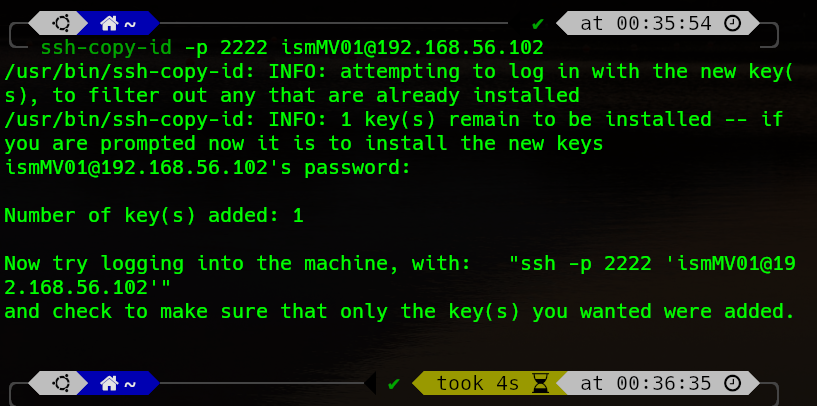
\includegraphics[width=\textwidth]{images/copiaLlave.png}
    \caption{SSH en mi máquina}
    \label{copiaLlave}
  \end{minipage}
  \hfill
  \begin{minipage}[b]{0.45\textwidth}
    \centering
    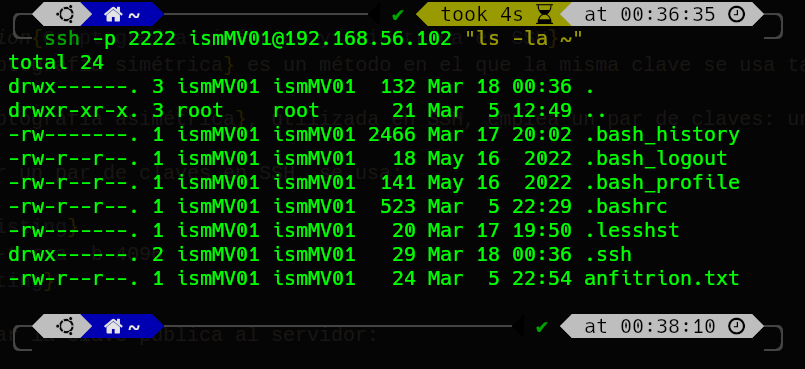
\includegraphics[width=\textwidth]{images/finalSSH.png}
    \caption{SSH final}
    \label{finalSSH}
  \end{minipage}
\end{figure}

\subsubsection*{Paso 6: Validar la conexión sin contraseña}

Para comprobar que el acceso es correcto, se ejecutará un comando remoto en la máquina virtual desde otro equipo o una máquina anfitriona. Se listará el contenido completo del directorio home del usuario remoto, incluidos los archivos ocultos (Ver Figura \ref{finalSSH}):

\begin{lstlisting}[style=mystyle]
ssh -p 2222 usuario@IP_del_Servidor "ls -la ~"
\end{lstlisting}

Si todo está configurado correctamente, el comando mostrará los archivos del directorio home sin requerir contraseña.





